\documentclass[14pt]{extbook}
\usepackage{multicol, enumerate, enumitem, hyperref, color, soul, setspace, parskip, fancyhdr} %General Packages
\usepackage{amssymb, amsthm, amsmath, latexsym, units, mathtools} %Math Packages
\everymath{\displaystyle} %All math in Display Style
% Packages with additional options
\usepackage[headsep=0.5cm,headheight=12pt, left=1 in,right= 1 in,top= 1 in,bottom= 1 in]{geometry}
\usepackage[usenames,dvipsnames]{xcolor}
\usepackage{dashrule}  % Package to use the command below to create lines between items
\newcommand{\litem}[1]{\item#1\hspace*{-1cm}\rule{\textwidth}{0.4pt}}
\pagestyle{fancy}
\lhead{Progress Quiz 6}
\chead{}
\rhead{Version B}
\lfoot{9689-6866}
\cfoot{}
\rfoot{Spring 2021}
\begin{document}

\begin{enumerate}
\litem{
Solve the rational equation below. Then, choose the interval(s) that the solution(s) belongs to.\[ \frac{7x}{-2x -6} + \frac{-2x^{2}}{4x^{2} +26 x + 42} = \frac{7}{-2x -7} \]\begin{enumerate}[label=\Alph*.]
\item \( \text{All solutions lead to invalid or complex values in the equation.} \)
\item \( x_1 \in [-0.96, 2.07] \text{ and } x_2 \in [-3.12,-3.03] \)
\item \( x \in [-3.17,-2.84] \)
\item \( x_1 \in [-0.96, 2.07] \text{ and } x_2 \in [-3.02,-2.99] \)
\item \( x \in [-4.26,-3.23] \)

\end{enumerate} }
\litem{
Determine the domain of the function below.\[ f(x) = \frac{4}{15x^{2} -42 x + 24} \]\begin{enumerate}[label=\Alph*.]
\item \( \text{All Real numbers except } x = a, \text{ where } a \in [0.4, 1] \)
\item \( \text{All Real numbers.} \)
\item \( \text{All Real numbers except } x = a \text{ and } x = b, \text{ where } a \in [17.7, 19.4] \text{ and } b \in [19.7, 20.7] \)
\item \( \text{All Real numbers except } x = a \text{ and } x = b, \text{ where } a \in [0.4, 1] \text{ and } b \in [1.6, 2.5] \)
\item \( \text{All Real numbers except } x = a, \text{ where } a \in [17.7, 19.4] \)

\end{enumerate} }
\litem{
Choose the graph of the equation below.\[ f(x) = \frac{-1}{x - 2} - 2 \]\begin{enumerate}[label=\Alph*.]
\begin{multicols}{2}\item 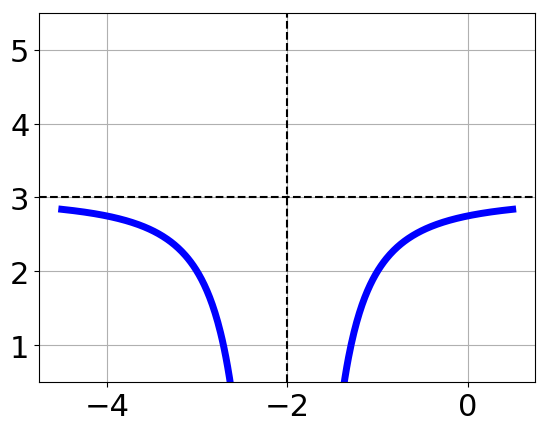
\includegraphics[width = 0.3\textwidth]{../Figures/rationalEquationToGraphAB.png}\item 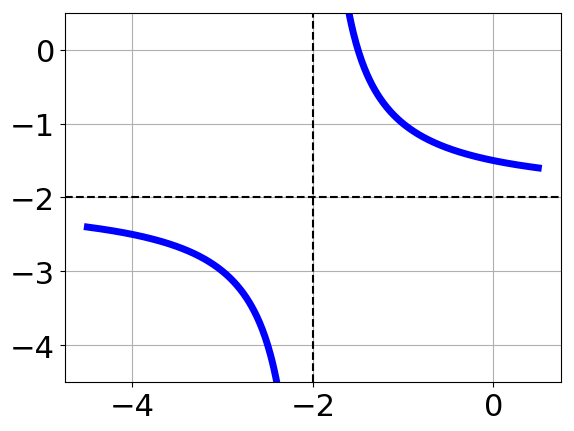
\includegraphics[width = 0.3\textwidth]{../Figures/rationalEquationToGraphBB.png}\item 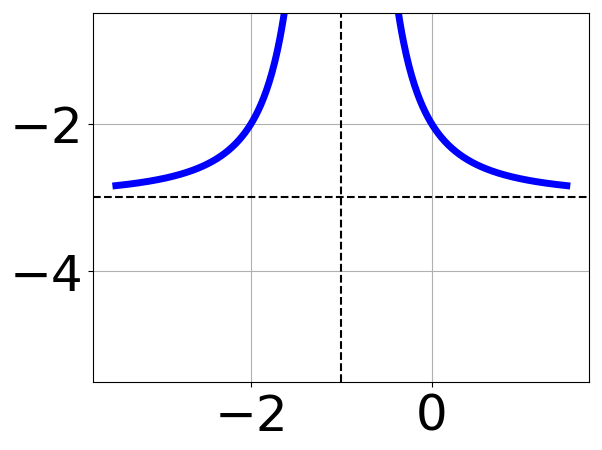
\includegraphics[width = 0.3\textwidth]{../Figures/rationalEquationToGraphCB.png}\item 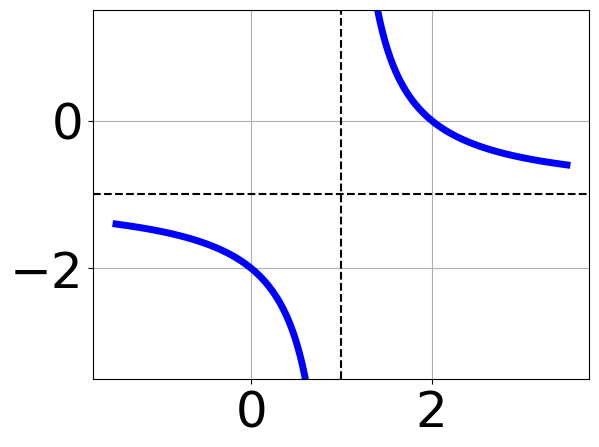
\includegraphics[width = 0.3\textwidth]{../Figures/rationalEquationToGraphDB.png}\end{multicols}\item None of the above.
\end{enumerate} }
\litem{
Choose the graph of the equation below.\[ f(x) = \frac{1}{x - 1} - 3 \]\begin{enumerate}[label=\Alph*.]
\begin{multicols}{2}\item 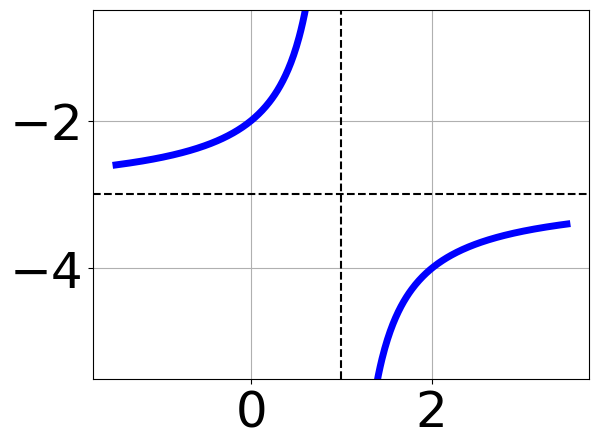
\includegraphics[width = 0.3\textwidth]{../Figures/rationalEquationToGraphCopyAB.png}\item 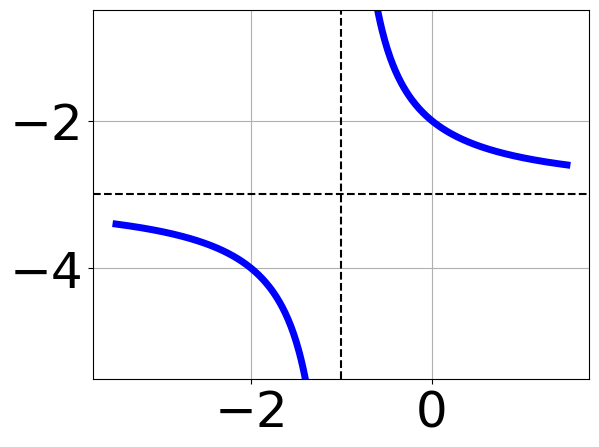
\includegraphics[width = 0.3\textwidth]{../Figures/rationalEquationToGraphCopyBB.png}\item 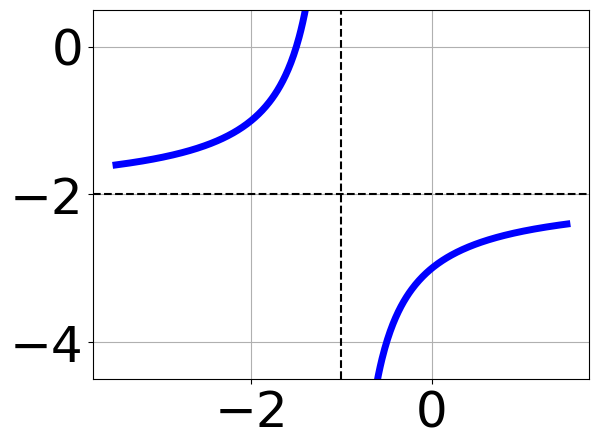
\includegraphics[width = 0.3\textwidth]{../Figures/rationalEquationToGraphCopyCB.png}\item 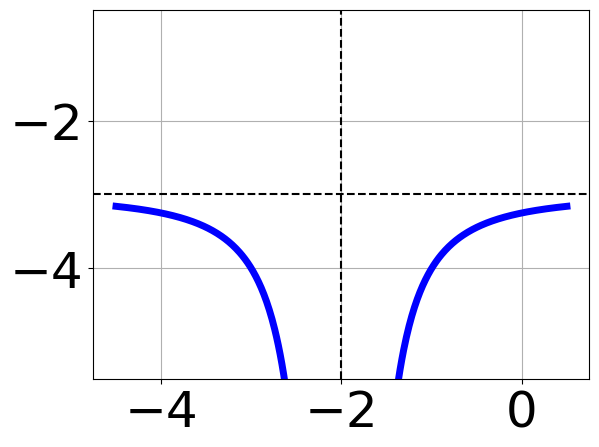
\includegraphics[width = 0.3\textwidth]{../Figures/rationalEquationToGraphCopyDB.png}\end{multicols}\item None of the above.
\end{enumerate} }
\litem{
Choose the equation of the function graphed below.
\begin{center}
    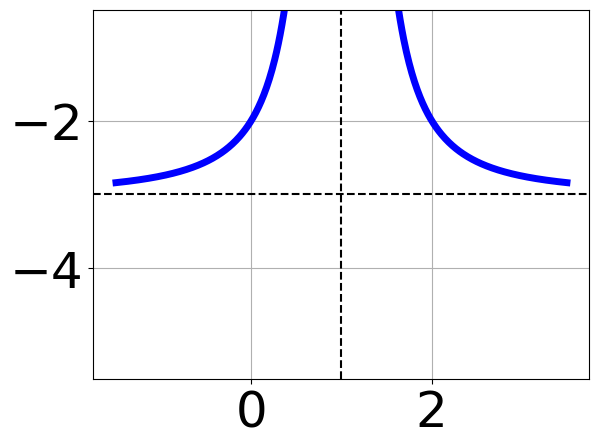
\includegraphics[width=0.5\textwidth]{../Figures/rationalGraphToEquationB.png}
\end{center}
\begin{enumerate}[label=\Alph*.]
\item \( f(x) = \frac{1}{(x - 1)^2} - 3 \)
\item \( f(x) = \frac{-1}{(x + 1)^2} - 3 \)
\item \( f(x) = \frac{1}{x - 1} - 3 \)
\item \( f(x) = \frac{-1}{x + 1} - 3 \)
\item \( \text{None of the above} \)

\end{enumerate} }
\litem{
Choose the equation of the function graphed below.
\begin{center}
    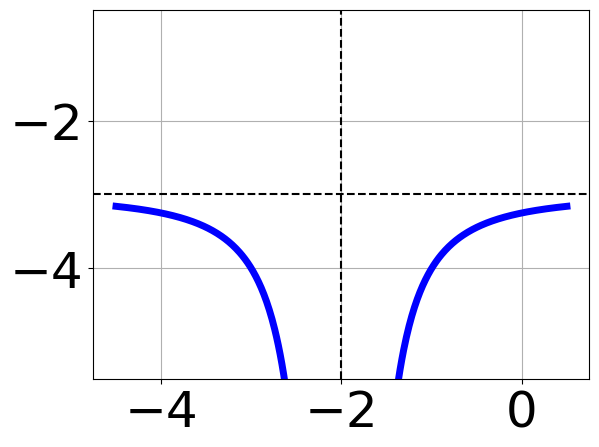
\includegraphics[width=0.5\textwidth]{../Figures/rationalGraphToEquationCopyB.png}
\end{center}
\begin{enumerate}[label=\Alph*.]
\item \( f(x) = \frac{-1}{x - 2} - 6 \)
\item \( f(x) = \frac{1}{x + 2} - 6 \)
\item \( f(x) = \frac{-1}{(x - 2)^2} - 6 \)
\item \( f(x) = \frac{1}{(x + 2)^2} - 6 \)
\item \( \text{None of the above} \)

\end{enumerate} }
\litem{
Solve the rational equation below. Then, choose the interval(s) that the solution(s) belongs to.\[ \frac{-5}{8x -7} + 6 = \frac{3}{-56x + 49} \]\begin{enumerate}[label=\Alph*.]
\item \( \text{All solutions lead to invalid or complex values in the equation.} \)
\item \( x_1 \in [-0.78, 0.22] \text{ and } x_2 \in [0.84,1.04] \)
\item \( x \in [-0.78,0.22] \)
\item \( x_1 \in [-0.03, 1.97] \text{ and } x_2 \in [0.98,1.14] \)
\item \( x \in [-0.03,1.97] \)

\end{enumerate} }
\litem{
Solve the rational equation below. Then, choose the interval(s) that the solution(s) belongs to.\[ \frac{3}{4x -5} + 7 = \frac{-9}{-16x + 20} \]\begin{enumerate}[label=\Alph*.]
\item \( \text{All solutions lead to invalid or complex values in the equation.} \)
\item \( x_1 \in [0.48, 0.92] \text{ and } x_2 \in [0.22,2.22] \)
\item \( x \in [1.22,2.22] \)
\item \( x_1 \in [-1.68, -0.96] \text{ and } x_2 \in [0.22,2.22] \)
\item \( x \in [-1.68,-0.96] \)

\end{enumerate} }
\litem{
Solve the rational equation below. Then, choose the interval(s) that the solution(s) belongs to.\[ \frac{-2x}{-4x + 2} + \frac{-4x^{2}}{16x^{2} +4 x -6} = \frac{-6}{-4x -3} \]\begin{enumerate}[label=\Alph*.]
\item \( x_1 \in [0.4, 1.3] \text{ and } x_2 \in [1.69,10.69] \)
\item \( x \in [-1.98,-0.23] \)
\item \( x \in [2.74,5.68] \)
\item \( x_1 \in [0.4, 1.3] \text{ and } x_2 \in [0.5,2.5] \)
\item \( \text{All solutions lead to invalid or complex values in the equation.} \)

\end{enumerate} }
\litem{
Determine the domain of the function below.\[ f(x) = \frac{5}{36x^{2} -60 x + 24} \]\begin{enumerate}[label=\Alph*.]
\item \( \text{All Real numbers except } x = a \text{ and } x = b, \text{ where } a \in [23.69, 24.49] \text{ and } b \in [35.81, 36.63] \)
\item \( \text{All Real numbers.} \)
\item \( \text{All Real numbers except } x = a, \text{ where } a \in [0.55, 0.88] \)
\item \( \text{All Real numbers except } x = a \text{ and } x = b, \text{ where } a \in [0.55, 0.88] \text{ and } b \in [0.96, 1.28] \)
\item \( \text{All Real numbers except } x = a, \text{ where } a \in [23.69, 24.49] \)

\end{enumerate} }
\end{enumerate}

\end{document}